\chapter{Random Forest and Bagging}
\label{ch-rforest}


This chapter
is based on Refs.\cite{wiki-bagging}
and \cite{wiki-rforest}.

Chapter \ref{ch-dtree}
defines decision trees (dtrees)
and explains how to construct them.
A Random Forest (RF) is 
an ensemble
of dtrees.
The RF algorithm is a
method of,
given a dataset,
constructing a RF
and averaging
over the classifier 
functions of the RF
to produce
an ensemble classifier.


The RF algo
uses  the method of 
Bootstrap Aggregating
(a.k.a. Bagging), which
is discussed in detail below.
Bagging
is a method
of constructing
an ensemble
of datasets (called {\bf bootstrap
datasets or bags})
that are 
fairly uncorrelated.
Each of
these bags is used to
train a {\bf bag-classifier}.
The bag-classifiers
are averaged over
to produce an {\bf
ensemble classifier,
or e-classifier} for short.
Bagging can be used
to
train any type
of bag-classifier,
but it was 
invented with
dtrees
in mind, 
and is still
 most commonly
used to train dtrees.

Boosting
(see Chapter \ref{ch-adaboost} on AdaBoost
and
Chapter \ref{ch-xgboost} on XGBoost)
is
another method,
besides Bagging,
of constructing a classifier function
from an ensemble 
of classifier functions.
These two methods are most commonly
applied to dtrees: Boosting for an ensemble of
small dtrees, and Bagging for a
random forest (which
is an ensemble
of dtrees that are 
usually much more
complicated than small dtrees).



\section{Bagging (with fully-featured bags)}
In this section
we discuss the bagging
algorithm.
As already 
mentioned,
bagging
is usually
used to train dtrees.
In this
section,
we explain bagging
in general,
not just for dtrees.


Let $L=[0,1,2, \ldots, nsam-1]$ be a list of
individuals (samples) in a population.
In this chapter, we will use the notation 
$A^\s=A[\s]$ 
and $\vec{A}=[A^\s:\s\in L]$
for a  list (vector, 1-D  array) indexed by $L$.
We will refer to $DS=(\vec{x}, \vec{y})$ 
where $x^\s\in val(\rvx)$, $y^\s\in val(\rvy)$,
as a dataset. If
$L_j$ is a list (possibly with 
duplicate items)
such that $set(L_j)\subset set(L)$,
 then
define
$DS_j=(\vec{x}, \vec{y})_{L_j}=
((x^\s)_{\s\in L_j}, 
(y^\s)_{\s\in L_j})$.
We will
refer to $DS_j$
as the {\bf restriction of 
$(\vec{x}, \vec{y})$ to $L_j$.}



We will refer to a function
$Y:val(\rvx) \rarrow val(\rvc)$
as a
classifier. It maps the vector of features $x\in val(\rvx)$
to a class $c\in val(\rvc)$. Below,
$Y_b$ for all $b$
and $Y_{ens}$
are classifiers.


\begin{figure}
$$
\xymatrix{
&
\rvL_0\ar[d]
&
\rvL_1\ar[d]
&
\rvL_2\ar[d]
&
\rvL_3\ar[d]
&
\rvL_4\ar[d]
\\
(\vec{\rvx},\vec{\rvy})
\ar[r]
\ar@/^1pc/[rr]
\ar@/^1pc/[rrr]
\ar@/^1pc/[rrrr]
\ar@/^1pc/[rrrrr]
&
(\vec{\rvx},\vec{\rvy})_{L_0}\ar[d]
&
(\vec{\rvx},\vec{\rvy})_{L_1}\ar[d]
&
(\vec{\rvx},\vec{\rvy})_{L_2}\ar[d]
&
(\vec{\rvx},\vec{\rvy})_{L_3}\ar[d]
&
(\vec{\rvx},\vec{\rvy})_{L_4}\ar[d]
\\
&
\rvY_0\ar[d]
&
\rvY_1\ar[dl]
&
\rvY_2\ar[dll]
&
\rvY_3\ar[dlll]
&
\rvY_4\ar[dllll]
\\
&
\rvY_{ens}
}
$$
\caption{Bnet for Random Forest (RF)
with 5 bags.}
\label{fig-rf-5-bags}
\end{figure}

Fig.\ref{fig-rf-5-bags}
is a bnet that encapsulates the RF algo.
The TPMs, printed in blue, for the
bnet Fig.\ref{fig-rf-5-bags},
are as follows.


Let $b\in\{0, 1, 2, \ldots, nbags-1\}=B$
and $\s\in L$. Let $L^\s_b\in L$ and
\beq\color{blue}
P(L_b^\s)=1/nsam
\eeq
In other words, each item in list $L_b$ 
is chosen from the items of list $L$, uniformly at random
with replacements.
 $|L_b|=|L|$ (same size as original).
$L_b$ can have duplicate items and be missing
items from $L$.

\beq\color{blue}
P((\vec{x}, \vec{y})_{L_b}|(\vec{x}, \vec{y}), L_b)
=
\indi(\;\;\;
(\vec{x}, \vec{y})_{L_b}= \text {restriction of }
(\vec{x}, \vec{y}) \text{ to }L_b
\;\;\;)
\eeq
We will refer to $(\vec{x}, \vec{y})$ as the
{\bf original dataset} and to
the $(\vec{x}, \vec{y})_{L_b}$
for $b\in B$
as the {\bf bootstrap datasets} or {\ {\bf bags}.

\beq\color{blue}
P(Y_b|(\vec{x}, \vec{y})_{L_b})=
\indi(\;\;\;
\text{$Y_b(\cdot)=$ 
classifier trained on dataset 
$(\vec{x},\vec{y})_{L_b}$.}
\;\;\;)
\eeq

\beq\color{blue}
P(Y_{ens}| (Y_b)_{b\in B})=
\prod_\s
\indi(
\;\;\;
Y_{ens}(x^\s)=
{\tt majority}(
\{Y_b(x^\s):b\in B\})
\;\;\;)
\eeq
The {\tt majority()}
function can be replaced
by an average $\frac{1}{nbags}\sum_b$
in case
the set of classes $val(\rvc)$
equals $\RR$ rather than a finite set.
We will refer to
$Y_{ens}$ as the {\bf ensemble
classifier (e-classifier)}
and to the $Y_b$
as the {\bf bag-classifiers}.


 


\begin{figure}[h!]
\centering
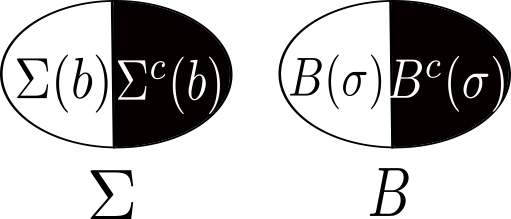
\includegraphics[width=2in]
{ran-forest/ran-forest-sets.png}
\caption
{$\Sigma(b)$ and $\Sigma^c(b)$
are disjoint sets whose union is $\Sigma$.
$B(\s)$ and $B^c(\s)$ 
are disjoint sets whose union is $B$.
} 
\label{fig-ran-forest-sets}
\end{figure}

Define 
(these definitions
are illustrated  in Fig.\ref{fig-ran-forest-sets})

\beq
\Sigma=set(L)\;,\;\;
\Sigma(b)=set(L_b)\;,\;\;
\Sigma^c(b)= \Sigma - \Sigma(b)
\eeq
and

\beq
B(\s)=\{b\in B: \s\in \Sigma(b)\}
\;,\;\;
B^c(\s)= B-B(\s)
\eeq
$\Sigma(b)$ is
the set of 
{\bf in-the-$b$-bag individuals}
and 
$\Sigma^c(b)$ is
the set of {\bf out-of-the-$b$-bag
 (OOB) individuals}. 
$B(\s)$
is the set of bags that
contain individual $\s$,
and $B^c(\s)$
is the set of bags that don't.

The {\bf OOB error} is defined as


\beq
err= \sum_{\s\in L} 
\indi(B^c(\s)\neq \emptyset)\indi(
\;\;\;y^\s\neq
{\tt majority}([Y_b(x^\s): b\in B^c(\s)])
\;\;\;)
\;.
\eeq
Empirical
results supposedly show that OOB error is comparable in 
accuracy to the error calculated
by doing cross-validation (CV)
 (see Chapter \ref{ch-cross-val}),
although CV error is considered
more dependable.

\section{Bagging (with randomly-shortened bags)}


Suppose the feature vector
$x^\s$ in the dataset $DS=(\vec{x},\vec{y})$
has $nf$ components; i.e., 
$x^\s=(x^\s_0, x^\s_1, \ldots, x^\s_{nf-1})\in
val(\rvx_0)\times val(\rvx_1)
\times\ldots\times val(\rvx_{nf-1})=val(\rvx)$.

For each bag $DS_b$,
one chooses at random
$nf'=\sqrt{nf}$
out of the $nf$  
features, and discards the remaining
features
from $DS_b$,
thus producing a new, 
{\bf randomly-shortened-bag (rs-bag)} $DS'_b$.
Each rs-bag 
is then used to train a bag-classifier,
usually a dtree, using the methods
for dtree SL  
described in Chapter \ref{ch-dtree}.
Using rs-bags
is called the {\bf random subspace method}.
The reason for using rs-bags
is that they further
decorrelate the set 
of bags used to train bag-classifiers.

